\section{Models and Methods}
\label{sec:models_and_methods}
\subsection{Dataset}
% Dataset citation: \citep{dernoncourt2017pubmed}
% See https://arxiv.org/pdf/1710.06071.pdf for description
% Pubmed 200k has a vocabulary size of 331k and contains 195,654 abstracts
% 200k: train has 190k abdstract (2.2M sentences), 2.5k validation (29k sentences), 2.5k test (29k sentences). Table in arxiv shows wrong number for test set but right number in text.

We evaluate our models on PubMed 200k RCT dataset \citep{dernoncourt2017pubmed} consisting of abstracts of biomedical literature for sequential sentence classification. This dataset consists of around 200,000 abstracts of randomized controlled trials which is around 2.3 million sentences split into ~98.7\% (2.24M) train and ~1.3\% (29.4K) test samples. The sentences are labeled according to their contribution in the abstract. The labels are: background, objective, methods, results, or conclusions [\autoref{listing:example_abstract}]. The dataset is slightly imbalanced with ~33\% sentences corresponding to 'methods' and ~35\% corresponding to 'results' labels. \autoref{fig:distributions} shows distribution of classes, distribution of tokens per sentence after preprocessing and distribution of characters per sentence.\\

% REMEMBER TO REFERENCE \autoref{fig:distributions} AND \autoref{listing:example_abstract} AND \autoref{listing:example_preprocess}

\begin{lstlisting}[frame=single, backgroundcolor=\color{light-gray}, basicstyle=\footnotesize\ttfamily,caption= {Example of one abstract from the PubMed 200k RCT dataset. Listing is inspired by \citet{dernoncourt2017pubmed}.},captionpos=b,label={listing:example_abstract}]
###25787999
BACKGROUND  Emotional eating in children has been   [...]
OBJECTIVE   We evaluated whether emotional eating   [...]
METHODS     Forty-one parent-child dyads were       [...]
RESULTS     Children at ages 5-7 y who were exposed [...]
RESULTS     Parents who reported the use of more    [...]
CONCLUSIONS Parents who overly control children 's  [...]
CONCLUSIONS Additional research is needed to        [...]
CONCLUSIONS This trial was registered at            [...]
\end{lstlisting}


\begin{figure*}[t]
    \centering
    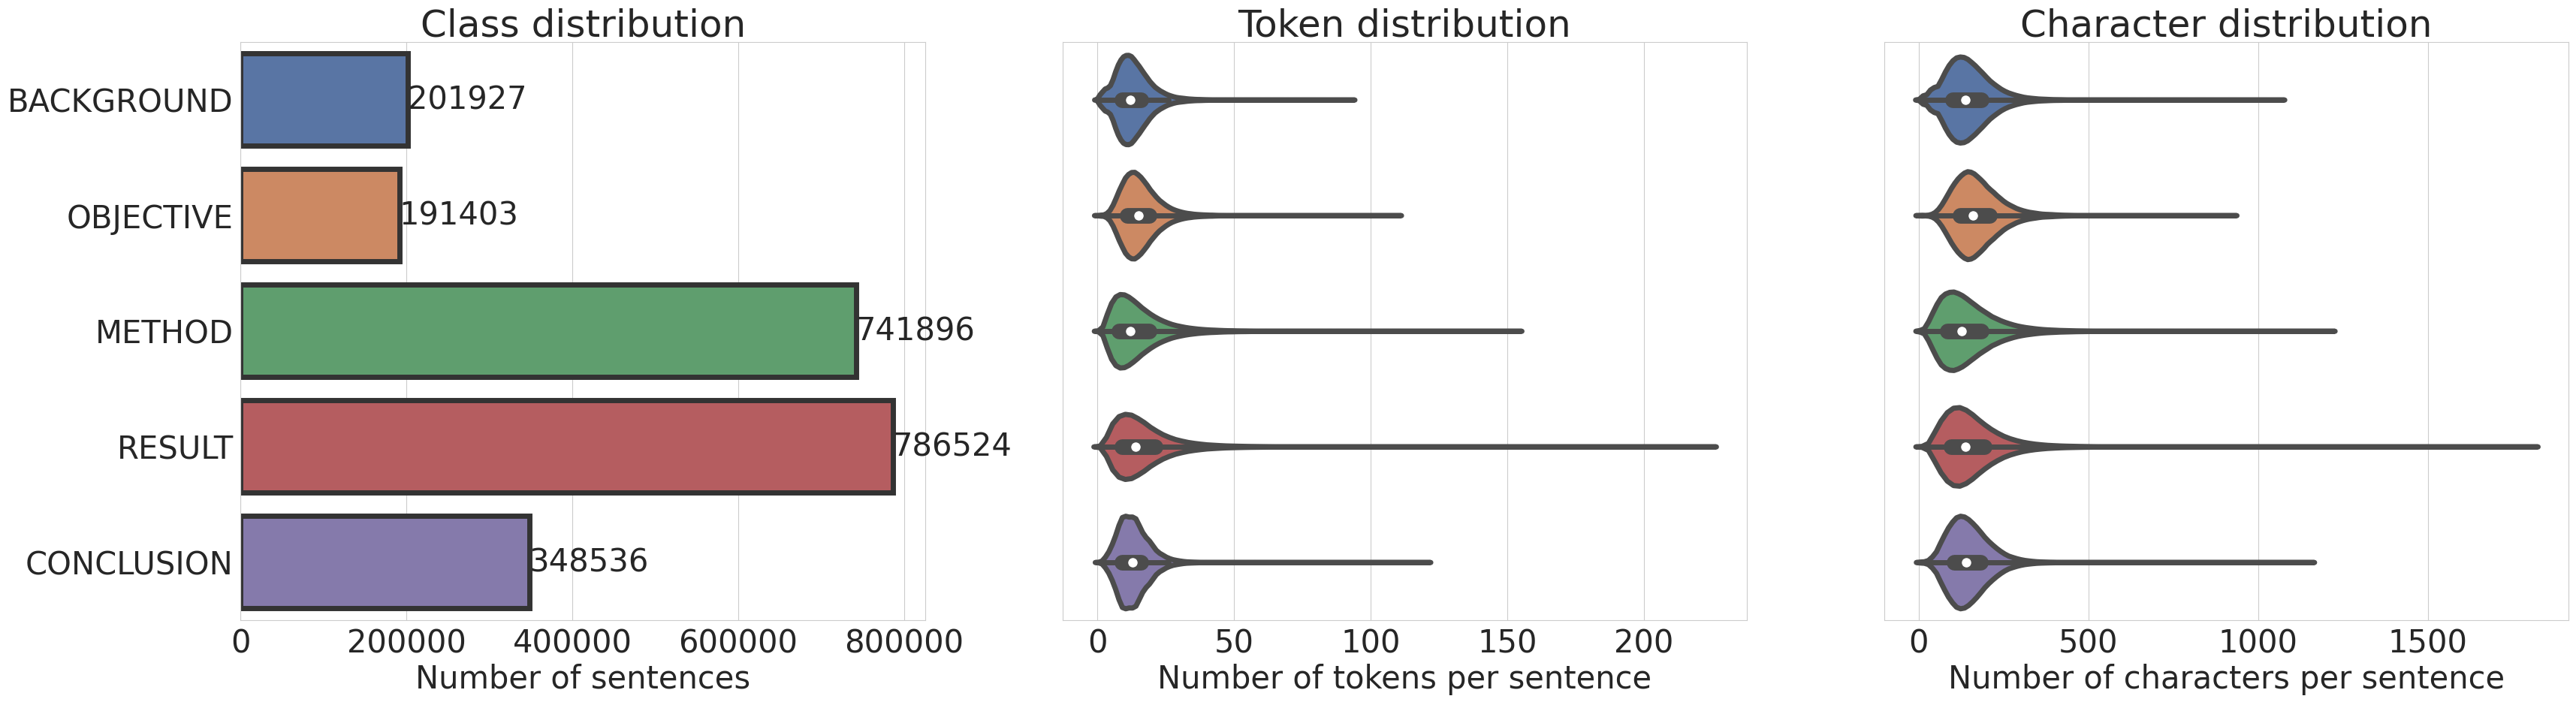
\includegraphics[width=0.70\textwidth]{figures/distributions_no_treshold.png}
    \caption{(Left) Distribution of classes. (Middle) Distribution of tokens per sentence after preprocessing sentences with lowercasing and removal of stop-words and punctuation. (Right) Distribution of characters per sentence.}
    \label{fig:distributions}
\end{figure*}


\subsection{Models}
We investigate several methods for obtaining sentence embeddings with varying complexity as well as explore the performance of different deep-learning and traditional ML classifiers. In the following we outline the models that we evaluate:

\begin{itemize}[leftmargin=0cm]
    \setlength\itemsep{0.6em}
    \item[]
    \textbf{Baseline:}
    As a baseline we employ a simple logistic regression classifier with term frequency-inverse document frequency (TF-IDF) features using both word-level unigrams and bigrams (\textsc{Baseline} and \textsc{Baseline w. lemmatization}).
    These models have the advantage of a low computation complexity while still showing reasonable performance on many NLP tasks and as such allows us to explore the trade-off between compute required and model performance.
    As a preprocessing step we lowercase our tokens, and remove stop-words and punctuation. We further introduce an optional lemmatization step [\autoref{listing:example_preprocess}].
    
    \item[]
    \textbf{One hot encoding:}
    As a second, simpler approach, we
     propose a \textsc{OneHot}, where each word is one hot encoded and the sentences are encoded as fixed-size arrays of one hot encoded words. Next, word embeddings are learned by an embedding layer which is followed by a three-layer MLP. To reduce computational cost, we limit the vocabulary size to 10k.

    % IF PREPROCESSING IS THE SAME AS IN THE BASELINE, REMEMBER TO WRITE IT!
    % word2vec citation: \citep{word2vec2013}
    % glove citation: \citep{pennington2014glove}
    \item[]
    \textbf{Word2Vec:}
    We apply the Word2Vec algorithm \citep{word2vec2013} to the given data after preprocessing using the same steps as in the baseline, to produce word embeddings. Sentence embeddings are then generated by averaging word vectors of all the words in the sentence. We train two classifiers on the sentence embeddings:\\
    \textsc{Word2Vec MLP:} We implement four dense layers with alternating Dropout layers in order to avoid overfitting.\\
    \textsc{Word2Vec LR:} We apply logistic regression to  the sentence embeddings to compare with the baseline.

    \item[]
    \textbf{GloVe:} As an alternative to Word2Vec, we use the GloVe embedding method which is able to incorporate global statistics \cite{pennington2014glove}. We follow the approach described above for Word2Vec. However, we don't train the GloVe embeddings on the given corpus but use Glove.6B provided by Pennington et al. \cite{pennington2014glove}.
    
    \item[]
    \textbf{BERT:} BERT models pre-trained on large corpora achieve state-of-the-art results in many NLP tasks \cite{devlin2018bert}. To explore whether they yield improvements in our setting, We use the Bio Clinical BERT model pre-trained on medical notes from the MIMIC III dataset by Alsentzer et al. \cite{alsentzer2019publicly, johnson2016mimic}. We investigate three different setups: \textsc{BERT Finetune} where we train the Bert model as well as a classification head and \textsc{BERT Freeze} where we freeze the BERT model and only train the final classifier. Instead of a single layer, the \textsc{BERT Freeze} classification head consists of a three-layer MLP which we find to improve performance when all previous layers are frozen. Further, to investigate whether the position/index of the sentence in the abstract 
    



\end{itemize}


\begin{lstlisting}[frame=single, backgroundcolor=\color{light-gray}, basicstyle=\footnotesize\ttfamily,caption= {Example of a sentence before preprocessing (original), after tokenization with lowercasing and removal of stop-words and punctuation, and after tokenization with lemmatization.},captionpos=b,label={listing:example_preprocess}]
ORIGINAL SENTENCE:
Participants said they were not sleeping more , but 
sleeping better , waking more refreshed , feeling less 
distressed about insomnia , and better able to cope when 
it occurred .

TOKENIZED (LOWERCASING, STOP-WORD & PUNCTUATION REMOVAL):
['participants', 'said', 'sleeping', 'sleeping', 'better',
'waking', 'refreshed', 'feeling', 'distressed', 'insomnia'
'better', 'able', 'cope', 'occurred']

TOKENIZED WITH LEMMATIZATION:
['participant', 'say', 'sleep', 'sleep', 'well',
'wake', 'refresh', 'feel', 'distressed', 'insomnia',
'well', 'able', 'cope', 'occur']
\end{lstlisting}




\begin{figure}
    % \centering
    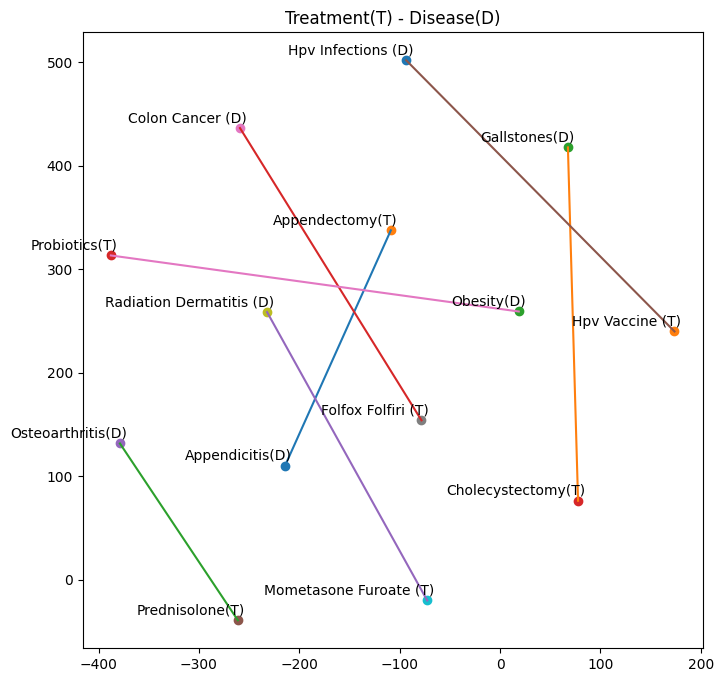
\includegraphics[width=0.40\textwidth]{figures/treatment_disease.png}
    \caption{Possible Treatment(T) for Disease(D): Relationship visualization of learned Word2Vec embeddings using t-SNE.}
    \label{fig:treatment-disease}
\end{figure}

\begin{figure}
    % \centering
    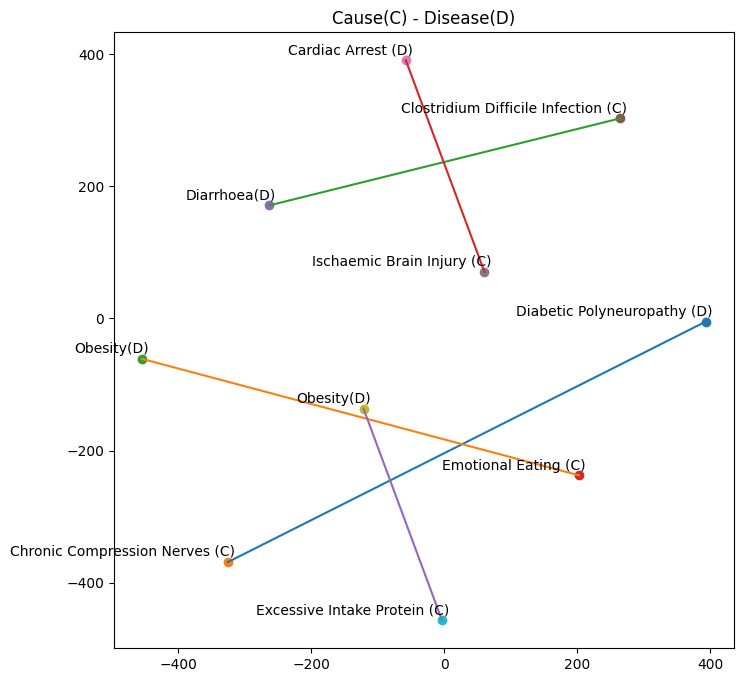
\includegraphics[width=0.40\textwidth]{figures/cause_disease.png}
    \caption{Possible Cause(C) of Disease(D): Relationship visualization of learned Word2Vec embeddings using t-SNE.}
    \label{fig:cause-disease}
\end{figure}


